\documentclass{article}

\usepackage{graphicx} % Required for inserting images
\usepackage[left=1in,right=1in,top=1in,bottom=1in]{geometry} \usepackage{amsmath}
\usepackage{amsthm} %proof environment
\usepackage{amssymb}
\usepackage{amsfonts}
\usepackage{enumitem} %nice lists
\usepackage{verbatim} %useful for something 
\usepackage{xcolor}
\usepackage{setspace}
\usepackage{titlesec}
\usepackage{blindtext} % I have no idea what this is 
\usepackage{caption}  % need this for unnumbered captions/figures
\usepackage{natbib}
\usepackage{tikz}
\usepackage{hyperref}

\titleformat{\section}{\bfseries\Large}{Problem \thesection:}{5pt}{}
\titleformat{\subsection}{\bfseries\large}{Subproblem \thesubsection:}{5pt}{}

\begin{document}

\title{AM 160 - SciML:}
\author{Dante Buhl}


\newcommand{\wrms}{w_{\text{rms}}}
\newcommand{\bs}[1]{\boldsymbol{#1}}
\newcommand{\tb}[1]{\textbf{#1}}
\newcommand{\bmp}[1]{\begin{minipage}{#1\textwidth}}
\newcommand{\emp}{\end{minipage}}
\newcommand{\R}{\mathbb{R}}
\newcommand{\C}{\mathbb{C}}
\newcommand{\N}{\mathcal{N}}
\newcommand{\K}{\bs{\mathrm{K}}}
\newcommand{\m}{\bs{\mu}_*}
\newcommand{\s}{\bs{\Sigma}_*}
\newcommand{\dt}{\Delta t}
\newcommand{\dx}{\Delta x}
\newcommand{\tr}[1]{\text{Tr}(#1)}
\newcommand{\Tr}[1]{\text{Tr}(#1)}
\newcommand{\Div}{\nabla \cdot}
\renewcommand{\div}{\nabla \cdot}
\newcommand{\Curl}{\nabla \times}
\newcommand{\Grad}{\nabla}
\newcommand{\grad}{\nabla}
\newcommand{\grads}{\nabla_s}
\newcommand{\gradf}{\nabla_f}
\newcommand{\xs}{x_s}
\newcommand{\xf}{x_f}
\newcommand{\ts}{t_s}
\newcommand{\tf}{t_f}
\newcommand{\pt}{\partial t}
\newcommand{\pz}{\partial z}
\newcommand{\uvec}{\bs{u}}
\newcommand{\F}{\bs{F}}
\newcommand{\T}{\tilde{T}}
\newcommand{\ez}{\bs{e}_z}
\newcommand{\ex}{\bs{e}_x}
\newcommand{\ey}{\bs{e}_y}
\newcommand{\eo}{\bs{e}_{\bs{\Omega}}}
\newcommand{\ppt}[1]{\frac{\partial #1}{\partial t}}
\newcommand{\DDt}[1]{\frac{D #1}{D t}}
\newcommand{\ppts}[1]{\frac{\partial #1}{\partial t_s}}
\newcommand{\pptf}[1]{\frac{\partial #1}{\partial t_f}}
\newcommand{\ppz}[1]{\frac{\partial #1}{\partial z}}
\newcommand{\ddz}[1]{\frac{d #1}{d z}}
\newcommand{\ppzetas}[1]{\frac{\partial^2 #1}{\partial \zeta^2}}
\newcommand{\ppzs}[1]{\frac{\partial #1}{\partial z_s}}
\newcommand{\ppzf}[1]{\frac{\partial #1}{\partial z_f}}
\newcommand{\ppx}[1]{\frac{\partial #1}{\partial x}}
\newcommand{\ppxi}[1]{\frac{\partial #1}{\partial x_i}}
\newcommand{\ppxj}[1]{\frac{\partial #1}{\partial x_j}}
\newcommand{\ppy}[1]{\frac{\partial #1}{\partial y}}
\newcommand{\ppzeta}[1]{\frac{\partial #1}{\partial \zeta}}


\maketitle 
% This line removes the automatic indentation on new paragraphs
\setlength{\parindent}{0pt}
\doublespacing

\setcounter{section}{1}
\section{}

\begin{enumerate}
    \item \textbf{\Large Perform SINDy for the noisy Lorenz 63 system.}

    I performed the SINDy algorithm for the lorenz system. I added noise to the
    derivative at each point according to the gaussian normal distribution with
    mean 0 and variance given by the problem set. In order to learn these
    coefficients, I merely used an rk4 integrator to find a trajectory and then
    computed the derivatives are each point along that trajectory. Then using
    a least squares solver, an solution for the coefficients is found. Finally,
    we iterate the least squares solution in order to neglect terms whose found
    coefficients are low (this algorithm doesn't take into account the relative
    weight of each column vector in the feature matrix which would be a vast
    improvement to the algorithm). Testing for the number of iterations used in
    the sindy algorithm can be seen by the plot shown in Figure
    \ref{fig:noisy_sindy}. 

    \begin{figure}[ht]
        \centering
        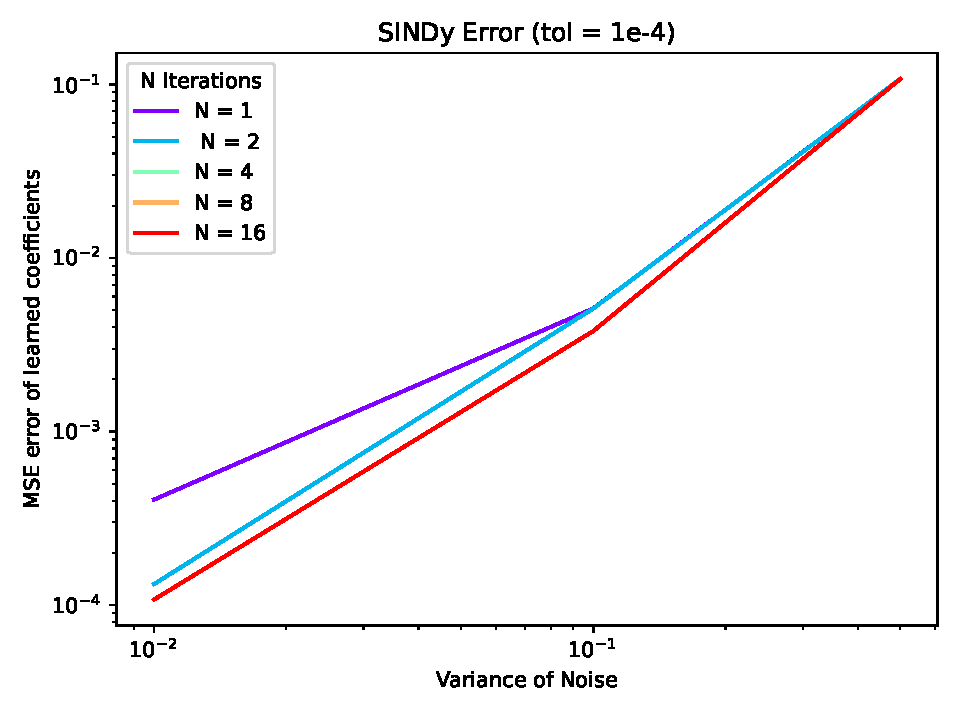
\includegraphics[width=.8\textwidth]{noisy_coeff_err.pdf}
        \caption{Plot of the MSE error for the learned coefficients
        ($\sqrt{(\theta_{\text{act}} - \theta_{\text{sindy}})^2}$) for the SINDy
        algorithm with a cutoff tolerance of $10^{-4}$. A different
        number of iterations was used and this is depicted in color. There seems
        to be no distinction between the learned coefficients after about 2
        iterations as $N = 4, 8, 16$ overlap exactly.}
        \label{fig:noisy_sindy}
    \end{figure}

    \item \textbf{\Large Perform SINDy on the Lorenz 63 system using derivative
    schemes}

    We can see from Figure \ref{fig:numerical_sindy} that more accurate
    derivative schemes enable SINDy to learn the coefficients better. Derivative
    schemes intrinsically contain errors bounded by the grid size and
    discretization. Notice that the higher order derivative scheme BDF3 allows
    the SINDy algorithm to better approximate the coefficients for the lorentz
    system compared to the first order centered finite difference scheme. I
    presume that with higher order derivative schemes and smaller grid sizes
    would decrease the error in the computed derivatives that SINDy learns from
    (which follows from any standard numerical methods course). 
    The choice in numerical method to prepare data for SINDy is, therefore, very
    important for bounding the error of the learned coefficients. We notice that
    the number of iterations doesn't appear to have a large effect on the
    learned coefficients either. For each derivative scheme, five iteration
    counts are used and show no visible change in the error on the plot as a
    function of number of iterations. 
    \begin{figure}[ht]
        \centering
        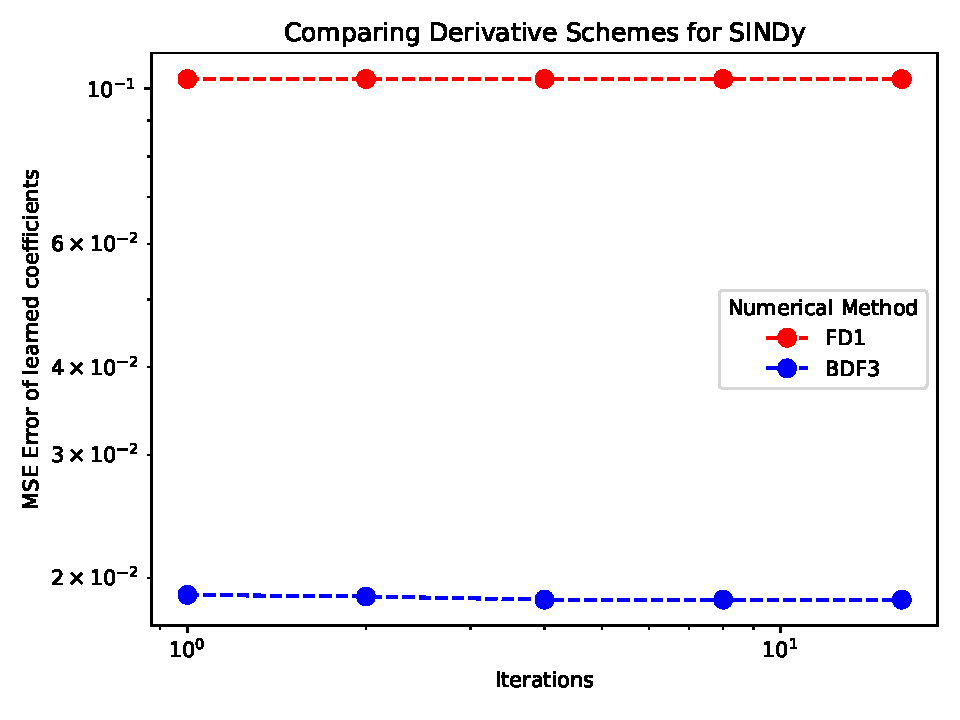
\includegraphics[width=.8\textwidth]{numerical_coeff_err.pdf}
        \caption{Plot of the MSE error for the learned coefficients
        ($\sqrt{(\theta_{\text{act}} - \theta_{\text{sindy}})^2}$) for the SINDy
        algorithm with the same number and cutoff tolerance as in Figure
        \ref{fig:noisy_sindy}, but this time instead of sets of noisy data, we
        perform sindy on numerically computed derivative schemes and compare the
        error}
        \label{fig:numerical_sindy}
    \end{figure}    
   
    \end{enumerate}
\end{document}
